\section{Overview of ILC and SaUCy}
\label{sec:background}

We tour the universal composability framework and give a flavor of ILC and SaUCy
with a simple example of how two untrusting parties, Alice and Bob, can securely
flip a coin using a commitment scheme.

\begin{figure*}[t]
\centering
\begin{tabular}{c|c}
\begin{subfigure}{.575\textwidth}
    $\Func_{\textsc{com}}$ proceeds as follows, running with parties $A$ and
  $B$.
    \begin{enumerate}
        \item Upon receiving a message $(\mathsf{Commit}, b)$ from $A$, where $b
          \in \{ 0, 1 \}$, record the value $b$ and send the message
          $(\mathsf{Receipt})$ to $B$. Ignore any subsequent \textsf{Commit}
          messages.
        \item Upon receiving a message $(\mathsf{Open})$ from $A$, proceed as
          follows: If some value $b$ was previously recorded, then send the
          message $(\mathsf{Open}, b)$ to $B$ and halt. Otherwise, halt.
    \end{enumerate}
\label{func:com}
\end{subfigure}\hspace{0.02\textwidth}
&\hspace{0.02\textwidth}
\begin{subfigure}{.35\textwidth}
  \lstinputlisting[style=myilc]{listings/Fcom.ilc}
\end{subfigure}
\end{tabular}
\caption{An ideal functionality for a one-time commitment scheme in prose (left)
  and in ILC (right).}
\label{func:com}
\end{figure*}

\subsection{Ideal Functionalities}
\label{subsec:functionalities}

Security in the UC framework is based on the real/ideal
paradigm~\cite{goldreich1987play}. To carry out some cryptographic task in the
real world, a set of parties must execute a protocol for the task among
themselves in a distributed fashion. In the ideal world, however, the parties
securely access an \emph{ideal functionality} $\mc{F}$, which is imagined as an
incorruptible trusted third party that securely (by construction) carries out
the task to be achieved by the protocol. The idea is that $\mc{F}$ obtains
inputs from the parties, carries out the task locally, and returns outputs back
to the parties. This serves as a self-contained specification
for the task's security requirements.\smallskip

\myheader{Example: Secure coin flipping.} Suppose two untrusting parties, Alice
and Bob, wish to securely flip a coin---Alice calls the coin flip by publishing $b
\in \{ 0, 1\}$, and Bob flips the coin by publishing $r \in \{0, 1\}$. If $b = r$,
then Alice wins; otherwise, Bob wins. Observe that simply having Alice and Bob
publish their respective values is not secure. If Alice publishes $b$ first,
then Bob can cheat by manipulating $r$ in his favor (and vice versa)!

In order to carry out the coin flip securely, they can use a commitment
scheme~\cite{brassard1988minimum}. Alice first publishes a commitment $C =
\mathsf{com}(b)$ for her bit $b$, waits for Bob to publish $r$, and then opens
and publishes a bit $b' = \mathsf{open}(C)$. If $r = b'$, then Alice wins;
otherwise, Bob wins.  Now, in order for such a commitment scheme to be secure,
it should satisfy the \emph{hiding} property (i.e., $C$ hides $b$ from Bob, so
he cannot manipulate $r$ in his favor) and the \emph{binding} property (i.e.,
$b=b'$, so that Alice cannot change the committed value in her favor).\smallskip

\myheader{Commitment functionality.} We can capture both of these properties at
once by defining an ideal functionality $\Func_{\textsc{com}}$ for a (one-time)
commitment scheme as it would appear in the cryptography literature
(Figure~\ref{func:com}, left). Whereas Alice and Bob carry out the two-party
commitment scheme in the real world, in the ideal world, they trust
$\Func_{\textsc{com}}$ to carry it out for them, so the hiding and binding
properties hold trivially. Of course, in the real world, Alice and Bob would not
want to trust such a third party (if it even exists), so the hope is that the
commitment scheme they use is ``just as good as'' $\Func_{\textsc{com}}$.\smallskip

\myheader{Commitment functionality in ILC.} In Figure~\ref{func:com} (right), we
have written $\Func_{\textsc{com}}$ in ILC. The function \textsf{fCom} takes as
arguments a read channel \textsf{frA}, which receives messages from $A$, and a
write channel \textsf{toB}, which sends messages to $B$. Channels in ILC are
typed, so each channel communicates values of the sum type \textsf{Msg}. Recall
that read channels are linearly typed, so \textsf{frA} simply has type
\textsf{Rd Msg}. On the other hand, write channels are intuitionistically typed,
so \textsf{toB} has type \textsf{!(Wr Msg)}. The ! operator (pronounced ``bang!'')
indicates a linear type for which contraction or weakening may be used. Arrow
types and lollipop types in ILC carry a mode $m \in \{\Wm, \Rm, \Vm\}$ (write,
read, and value, respectively), but value modes are elided.

The function body of \textsf{fCom} closely follows the functionality
$\Func_{\textsc{com}}$, but several points are worth mentioning. First, we give
the typing rule for the expression $\eLetRd{x_1}{x_2}{e_1}{e_2}$:
\begin{mathpar}
\Infer{letrd}
{\Delta_1 ; \Gamma |- e_1 : \tyRd{A} |> R\\
\Delta_2,x_1:\tyBang{A},x_2:\tyRd{A} ; \Gamma |- e_2 : B |> m
}
{\Delta_1, \Delta_2 ; \Gamma |- \eLetRd{x_1}{x_2}{e_1}{e_2} : B |> R}
\end{mathpar}
The value read on the read channel from evaluating $e_1$ is bound as $x_1$ and
the read channel itself is rebound as $x_2$ so that it may be reused at a later
time. Typing judgements also yield modes, and the evaluation of $e_1$ yields a
mode $\Rm$. The evaluation of $e_2$, on the other hand, can yield any mode
$m$. However, the mode of the whole read expression is a mode $\Rm$. To be more
exact, it is the sequential composition of the elided mode $\Vm$ and $m$, i.e.,

The modes $m_1$ and $m_2$ of expressions $e_1$ and $e_2$ compose
sequentially to yield $m1 ;; m2 => m3$ (mode compositions are defined in
Section~\ref{sec:ilc}).
In \textsf{fCom}, pattern matching with the ! operator
unpacks linearly typed values, so the value bound to the $b$ in the first read
from \textsf{frA} has an intuitionistic type and can be used without
restriction.

Finally, evaluating \textsf{fCom} with appropriately typed arguments yields a
read mode computation that returns a value of type \textsf{!Unit}.

\subsection{UC Emulation}
\label{subsec:emulation}

We say that a protocol $\pi$ \emph{emulates} (or \emph{securely realizes})
$\mc{F}$ if any attack that is possible on $\pi$ is also possible on
$\mc{F}$. However, since $\mc{F}$ is designed to be secure by definition, such
an attack does not lead to a break in security.

Proving emulation formally proceeds in two steps. The first step is
constructive: We must construct a \emph{simulator} $\mc{S}$ (a simulated
adversary) that can emulate the attack of any adversary $\mc{A}$ on $\pi$, but
instead, on $\mc{F}$. The second step is a relational analysis: We must show
that running $\pi$ under attack by any adversary $\mc{A}$ (the real world) is
\emph{indistinguishable} from running $\mc{F}$ under attack by $\mc{S}$ (the
ideal world) to any distinguisher $\mc{Z}$, called the \emph{environment}. In
particular, $\mc{Z}$ is an interactive distinguisher: It interacts with the real
world and the ideal world in a well-defined manner, and the simulation is good
if no $\mc{Z}$ can distinguish between the two.

\begin{figure}
  \centering
  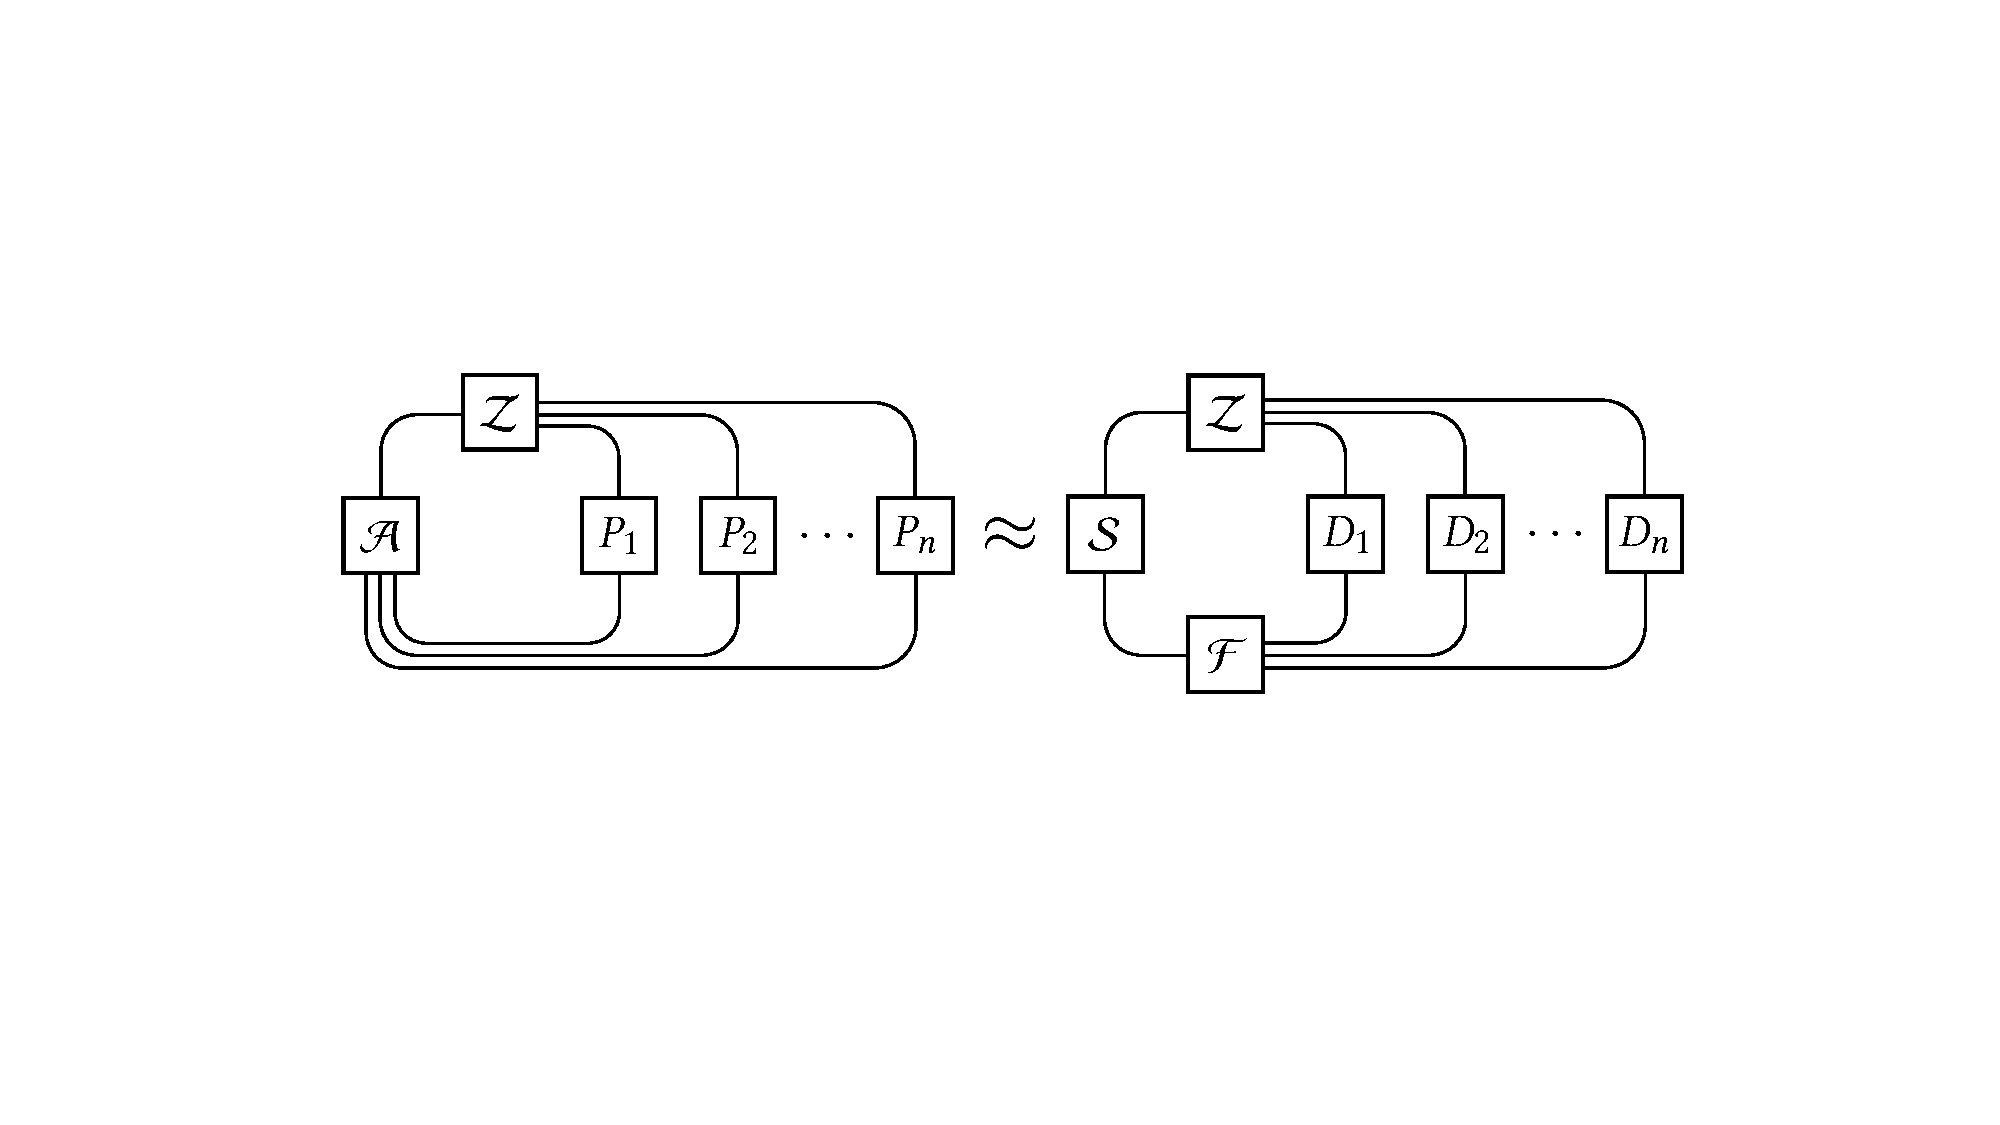
\includegraphics[width=\linewidth]{graphics/uc-experiment}
  \caption{UC experiment with real world (left) and ideal world (right).}
  \label{fig:uc-experiment}
\end{figure}

Figure~\ref{fig:uc-experiment} illustrates the UC experiment: connecting lines
denote communication channels,\footnote{Note that all communication passes
  through the adversary $\mc{A}$. In the bare model, communication is
  asynchronous, unauthenticated, and unreliable, but other models of
  communication can be built atop this model.} $P_1, P_2, \ldots, P_n$ represent
parties executing protocol $\pi$, and $D_1, D_2, \ldots, D_n$ represent ``dummy''
parties that simply relay information between the environment and the ideal
functionality.

\begin{comment}
\subsection{UC composition}
\label{subsec:composition}

The advantage of security definitions in UC is that they satisfy strong
composability guarantees, even under concurrent composition. Suppose that $\pi_1$
is a protocol that securely realizes a functionality $\mc{F}_1$. If a protocol
$\pi_2$, using $\mc{F}_1$ as a subroutine, securely realizes a functionality
$\mc{F}_2$, then the protocol $[\pi_1 / \mc{F}_1]\pi_2$, in which calls to
$\mc{F}_1$ are replaced by calls to $\pi_1$, also securely realizes
$\mc{F}_2$. That way, it suffices to analyze the security of the standalone
protocol $\pi_2$ in the $\mc{F}_1$-hybrid model, where parties run $\pi_2$ with
access to $\mc{F}_1$, as opposed to the composite protocol of $\pi_2$ and
$\pi_1$. Figure~\ref{fig:uc-composition} illustrates protocol composition. The
setup on the left represents the $\mc{F}_1$-hybrid model, and the setup on the
right represents the protocol substitution $[\pi_1 / \mc{F}_1]\pi_2$, which
maintains security.

\begin{figure}
  \centering
  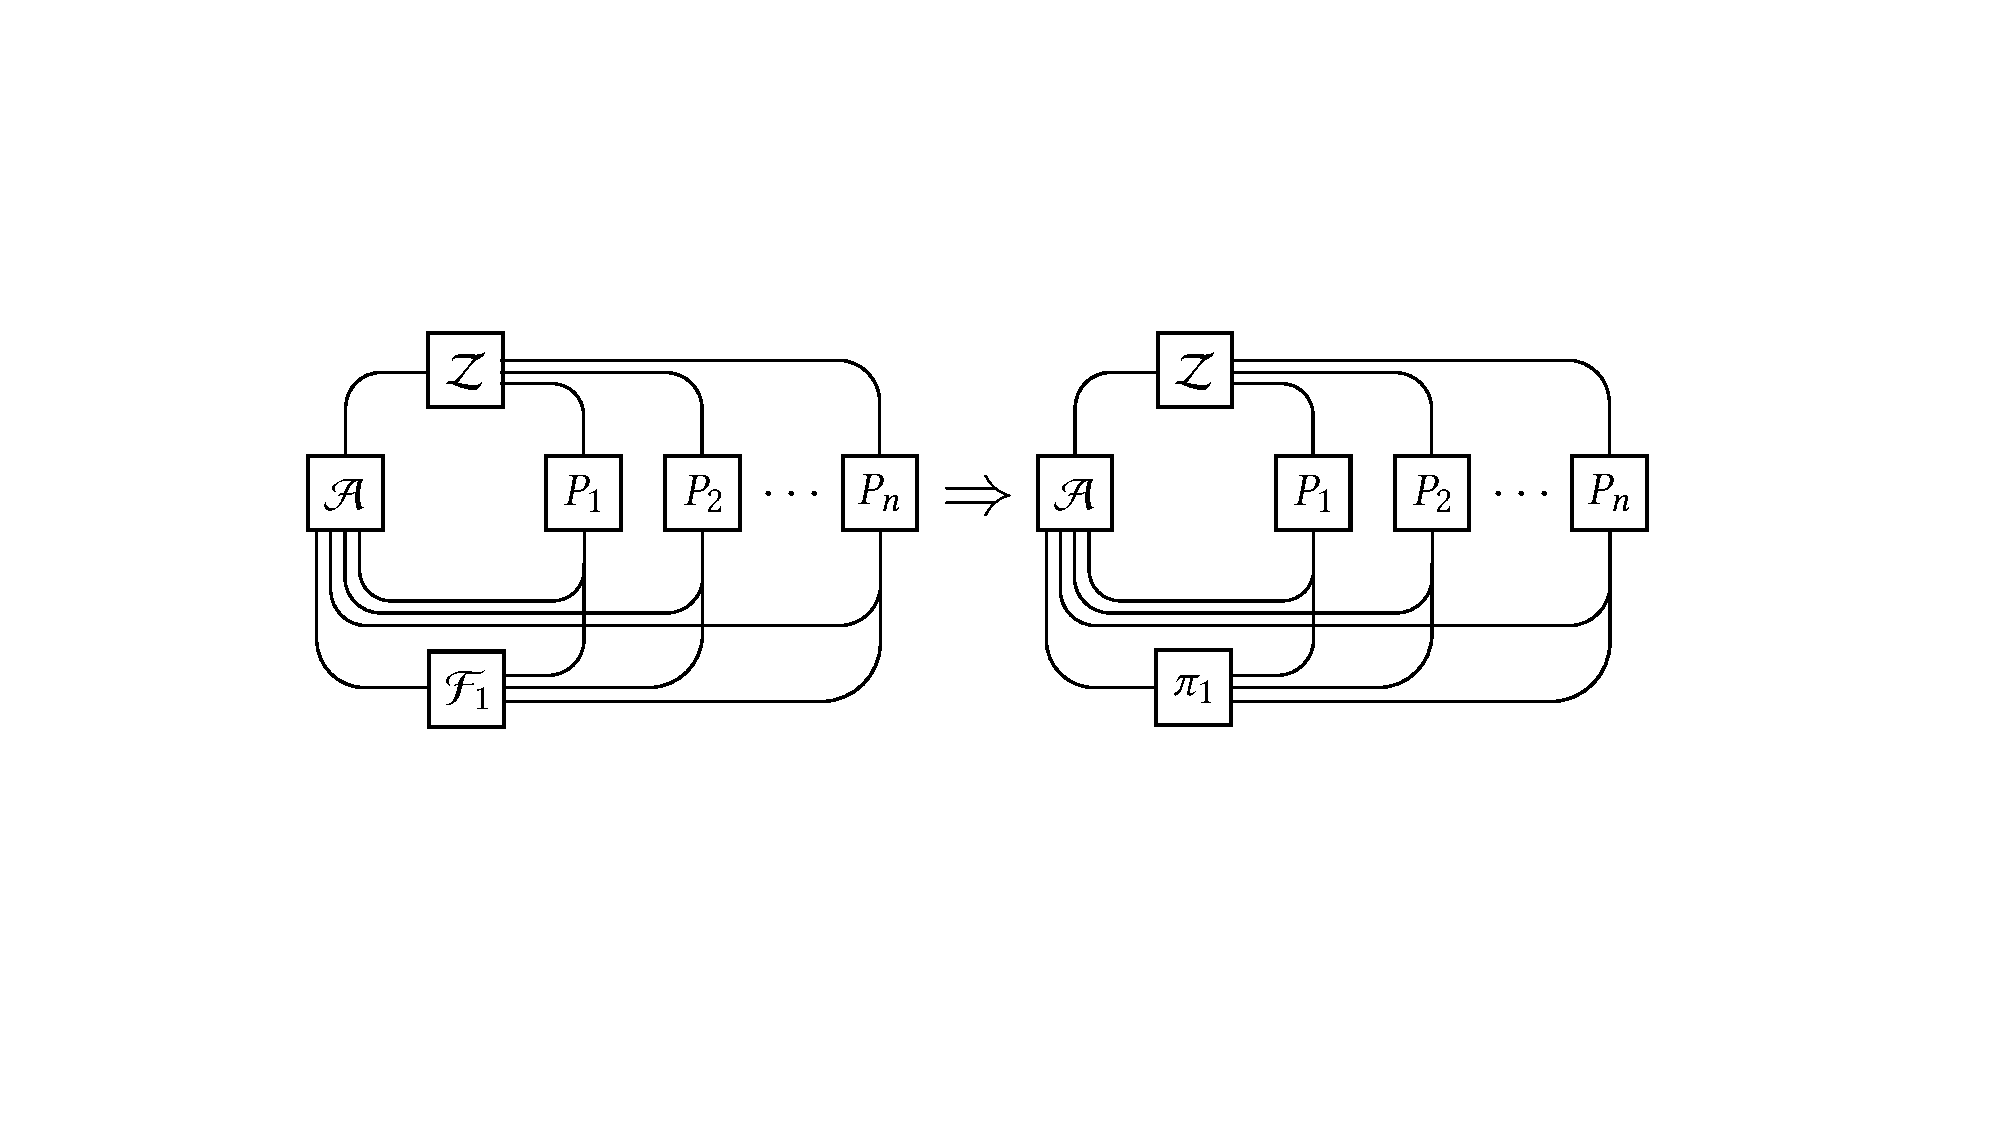
\includegraphics[width=\linewidth]{graphics/composition}
  \caption{UC protocol composition theorem.}
  \label{fig:uc-composition}
\end{figure}
\end{comment}
